\documentclass{beamer}

\usetheme{Boadilla}

\usepackage[utf8]{inputenc}
\usepackage[spanish]{babel}
\usepackage{physics}
\usepackage{tikz-cd}

\DeclareMathOperator{\SL}{SL}
\DeclareMathOperator{\GL}{GL}
\DeclareMathOperator{\Hom}{Hom}
\DeclareMathOperator{\id}{id}
\DeclareMathOperator{\SU}{SU}
\DeclareMathOperator{\SO}{SO}

\title[Física de partículas]{Simetría: partículas como representaciones del grupo de Poincaré}
\author[I. Burbano]{Iván Mauricio Burbano Aldana}
\institute[Uniandes]{Universidad de los Andes}

\begin{document}

\frame{\titlepage}

\begin{frame}
\frametitle{Tabla de Contenidos}
\tableofcontents
\end{frame}

\section{Transformaciones de Lorentz}

\begin{frame}
\frametitle{Espaciotiempo}
Un espaciotiempo relativista es \cite{Matolcsi1993} un par $(M,g)$ donde:
\begin{itemize}
\item $M$ es un espacio afín de 4 dimensiones modelado en un espacio vectorial $\vb{M}$;
\item $g:\vb{M}\times \vb{M}\rightarrow I\otimes I$ es una forma de Lorentz.
\end{itemize}
\end{frame}

\begin{frame}
\frametitle{Espaciotiempo aritmético}
\begin{alertblock}{Ejemplo}
$(\mathbb{R}^4,\eta)$ donde $\eta:\mathbb{R}^4\times\mathbb{R}^4\rightarrow\mathbb{R}$ en la base canónica
\begin{equation}
\eta_{ab} = \mqty[1 & 0 & 0 & 0 \\ 0 & -1 & 0 & 0 \\ 0 & 0 & -1 & 0 \\ 0 & 0 & 0 & -1]_{ab}
\end{equation}
Todo espaciotiempo es isomorfo a este pero no de manera canónica!
\end{alertblock}
\end{frame}

\begin{frame}
\frametitle{Grupo de Poincaré $\mathcal{P}$}
Transformaciones $\mathbb{R}^4\rightarrow\mathbb{R}^4$ que preservan la estructura espacio tiempo. Entonces deben ser:
\begin{itemize}
\item afines
\begin{align}
\begin{split}
\mathbb{R}^4\times \Hom(\mathbb{R}^4,\mathbb{R}^4) \ni(a,\Lambda):\mathbb{R}^4&\rightarrow\mathbb{R}^4 \\
p & \mapsto \Lambda p + a ;
\end{split}
\end{align}
\item ortogonales ($\Lambda\in \mathcal{L}$ el grupo de Lorentz)
\begin{equation}
\eta(u,v)=\eta(\Lambda u, \Lambda v).
\end{equation}
\end{itemize}
Como $\mathcal{L}$ actúa de manera natural sobre $\mathbb{R}^4$ la estructura de grupo es la de producto semidirecto
\begin{align}
\begin{split}
\mathcal{P} = \mathbb{R}^4&\rtimes \mathcal{L} \\
(a,\Lambda)(a',\Lambda')& = (a + \Lambda a', \Lambda\Lambda ')
\end{split}
\end{align}
\end{frame}

\begin{frame}
\frametitle{Transformaciones ortocronas propias}
Podemos clasificar a las transformaciones de Lorentz por \cite{Scheck2010}
\begin{center}
\begin{tabular}{|c|c|c|}
\hline
Componente conexa & $\det \Lambda$ & $\Lambda^0_0$ \\
\hline
$\mathcal{L}_+^\uparrow$ & $1$ & $\geq 1$ \\ 
$\mathcal{L}_+^\downarrow = PT\mathcal{L}_+^\uparrow$ & $1$ & $\leq -1$ \\ 
$\mathcal{L}_-^\uparrow = P\mathcal{L}_+^\uparrow$ & $-1$ & $\geq 1$ \\ 
$\mathcal{L}_-^\downarrow = T \mathcal{L}_+^\uparrow$ & $-1$ & $\leq -1$ \\
\hline 
\end{tabular}
\end{center}
Como se vio en clase, el análisis de $P$ y $T$ debe hacerse con cuidado. Nos restringimos al grupo de Lorentz ortocrono propio $\mathcal{L}_+^\uparrow$ y al grupo de Poincaré correspondiente $\mathcal{P}_+^\uparrow = \mathbb{R}^4\rtimes \mathcal{L}_+^\uparrow$.
\end{frame}

\begin{frame}[fragile]
\frametitle{Recubridor Universal}
\begin{columns}
\column{0.58\textwidth}
\begin{figure}
\centering
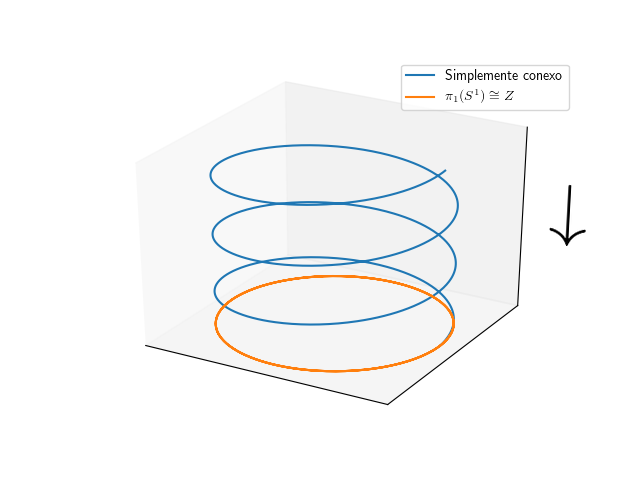
\includegraphics[width=\textwidth]{helice.png}
\caption{Se muestra como $\mathbb{R}$ es el recubridor universal de $S^1$.}
\end{figure}
\column{0.40\textwidth}
\begin{align}
\begin{split}
\Phi:\mathbb{R}^4&\rightarrow \Hom(\mathbb{C}^2,\mathbb{C}^2)_s \\
v^\alpha e_\alpha&\mapsto v^\alpha\sigma_\alpha \\
\end{split}
\end{align}
\begin{equation}
\eta(u,u)=\det(\Phi(u))
\end{equation}
\begin{equation}
\Lambda:\SL(\mathbb{C}^2)\rightarrow \mathcal{L}^+_\uparrow
\end{equation}
\end{columns}
\end{frame}

\section{Grupos de Simetría en Mecánica Cuántica}

\begin{frame}
\frametitle{Simetrías en mecánica cuántica}
\begin{itemize}
\item Estados puros y observables básicos: Proyecciones $\rho_\psi$ sobre el subespacio generado por $\psi\in\mathcal{H}$
\item Probabilidad de transición de $\rho_\phi$ a $\rho_\psi$ es $\tr(\rho_\psi\rho_\phi)=\frac{|\langle\phi,\psi\rangle|^2}{\|\phi\|^2\|\psi\|^2}$
\item Las simetrías de un sistema están representadas por grupos $G$ que actuan sobre el espacio de estados mediante una representación $T$ tal que se preservan estas probabilidades, es decir, para todo $g\in G$
\begin{equation}
\tr(T(g)(\rho_\psi)T(g)(\rho_\phi))=\tr(\rho_\psi\rho_\phi).
\end{equation} 
\end{itemize}
\end{frame}

\begin{frame}
\frametitle{Importancia del recubridor fundamental}
\begin{itemize}
\item ¡Es difícil trabajar con esta clase de mapas! Sería mejor poder trabajar con mapas entre vectores
\item Para cierto grupos $G$, como el de Poincaré, se puede demostrar que cualquier representación como la descrita arriba viene de una representación unitaria $U:\tilde{G}\rightarrow U(\mathcal{H})$ del recubridor universal $\tilde{G}$.
\item Solo tenemos que hallar representaciones unitarias de $\mathbb{R}^4\rtimes\SL(\mathbb{C}^2)$.
\end{itemize}
\end{frame}

\section{Representaciones irreducibles del grupo de Poincaré}

\begin{frame}
\frametitle{Rol de la energía-momento}
Como tenemos representaciones unitarias, existe, operadores autoadjuntos $P_a$ que generan traslaciones
\begin{equation}
U(a,\id_{\mathbb{C}^2})=e^{ia^bP_b}.
\end{equation}
Como las traslaciones conmutan, los generadores deben conmutar también. Además, transforman como cuadrivectores
\begin{equation}
U(0,\alpha)^{-1}P^a U(0,\alpha) = \Lambda(\alpha)^a_b P^b.
\end{equation}
Entonces adquieren la interpretación de los operadores de energía momento. Las representaciones irreducibles van a estar etiquetadas por los subespacios propios que corresponden a $p$ y que podemos conectar mediante $\mathcal{P}^+_\uparrow$.
\end{frame}

\begin{frame}
\frametitle{Programa}
El esquema general va a ser\cite{Sternberg1994}
\begin{itemize}
\item hallar las orbitas de la acción de $\SL(\mathbb{C}^2)$;
\item hallar el grupo de isotropía de un punto en cada órbita;
\item entontrar las representaciones irreducibles de este.
\end{itemize}
\end{frame}

\begin{frame}
\frametitle{Orbitas de la acción de $\SL(\mathbb{C}^2)$}
\cite{Haag1992}
\begin{center}
\begin{tabular}{|c|c|}
\hline
clase & órbita \\
\hline
$m_+$ & $\eta(p,p)=m^2$ y $p^0>0$ \\
$0_+$ & $\eta(p,p)=0$ y $p^0\geq 0 $ \\
$0_0$ & $p=0$ \\
$\kappa$ & $\eta(p,p)=-\kappa^2$ \\
$m_-$ & $\eta(p,p)=m^2$ y $p^0<0$ \\
$0_-$ & $\eta(p,p)=0$ y $p^0\leq 0$ \\
\hline
\end{tabular}
\end{center}
\end{frame}

\begin{frame}
\frametitle{Estudio de $m_+$}
Veamos el ejemplo de $m_+$ y como nos podemos mover a través de ella. Escoja $\overline{p}=(m,0,0,0)$ y defina para todo $p$ tal que $\eta(p,p)=m^2$ y $p^0>0$
\begin{equation}
\beta(p)=\left(\frac{E_p\id_{\mathbb{C}^2}+\sum_{\mu=1}^3p^\mu\sigma_\mu}{m}\right)^{1/2}
\end{equation}
con $E_p=\sqrt{\sum_{\mu=1}^3(p^\mu)^2+m^2}=p^0$. Luego 
\begin{equation}
\Lambda(\beta(p))\overline{p} = p.
\end{equation}
\end{frame}

\begin{frame}
\frametitle{Grupo de isotropía}
El grupo de isotropía de $\overline{p}$ satisface
\begin{equation}
\overline{p} = \Lambda(\alpha)(\overline{p}) = \Phi^{-1}(\alpha\Phi(\overline{p})\alpha^*) = \Phi^{-1}(m\alpha\alpha^*)=m\Phi^{-1}(\alpha\alpha^*).
\end{equation} 
Concluimos que el grupo de isotropía es $\SU(\mathbb{C}^2)$ el recubridor universal de $\SO(\mathbb{R}^3)$.
\end{frame}

\begin{frame}
\frametitle{Clasificación en irreducibles}
Sabemos que las representaciones irreducibles de $\SU(\mathbb{C}^2)$ están etiquetadas por espín $s\in\mathbb{N}/2$\cite{Hall2013}. Luego las representaciones irreducibles de $\mathcal{P}^+_\uparrow$ están etiquetadas por una masa $m\in\mathbb{R}^+$ y espín $s\in\mathbb{N}/2$.
\end{frame}

\begin{frame}
\frametitle{Referencias}
\bibliography{/home/ivan/Documents/Bib_Files/particle_physics_2017_II}
\bibliographystyle{apalike}
\end{frame}

\end{document}